\documentclass[11pt,a4paper]{article}

\usepackage[margin=2.2cm]{geometry}
\usepackage{amsmath,amssymb}
\usepackage{graphicx}
\usepackage{booktabs}
\usepackage{listings}
\usepackage{xcolor}
\usepackage[hidelinks]{hyperref}
\usepackage{caption}
\usepackage[section]{placeins}
\captionsetup{font=small,labelfont=bf}

\lstset{basicstyle=\ttfamily\small,columns=fullflexible,keepspaces=true,
        frame=single,rulecolor=\color{gray!50},xleftmargin=1em,xrightmargin=1em}
\newcommand{\code}[1]{\texttt{#1}}

\title{Triangulating coastlines in glgrib\\[0.3em]
\large EarCut compared with constrained Delaunay triangulation (Triangle, CDT)\\
on GSHHS and Natural Earth}
\author{}
\date{2026-11-25}

\begin{document}
\sloppy
\maketitle

\begin{abstract}
glgrib triangulates its coastline polygons with an ear-cutting algorithm on the sphere
(\code{EarCut.cc}, described in \code{earcut.pdf}). This report compares it with constrained
Delaunay triangulation (CDT), using two implementations: J.~Shewchuk's \emph{Triangle} (non-free
licence, used only as a reference) and the \emph{CDT} library (MPL-2.0, usable in glgrib).
All methods were run on every GSHHS file shipped with glgrib and on Natural Earth, the data set used
by ECMWF Magics, with automatic checks of each result.
On valid rings, Triangle and CDT never failed and never produced an inverted triangle; EarCut
produced wrong triangulations in about 1 ring in 2\,300 at intermediate and high resolution,
mostly single inverted slivers, probably caused by single-precision arithmetic, and aborted on Natural Earth
10m land because of a new bug found in \code{getLatRange}. CDT is as fast as EarCut or faster,
gives much better-shaped triangles, and, with intersections forbidden, detects exactly the
invalid rings of the data. The main costs of adopting it are a projection to the plane and, for
invalid rings only, extra vertices.
\end{abstract}

\tableofcontents

\section{What was compared}

\subsection{Methods}

\begin{center}\small
\begin{tabular}{lll}
\toprule
name & what & notes \\
\midrule
EarCut & \code{EarCut::processRing} as in glgrib & OpenMP in rings of $\geq 300$ points \\
EarCut fixed & same code with $R^\top$ and serial passes & built from a \code{sed}'ed copy \\
Triangle & Triangle 1.6, switches \code{-pzQBP} & also run with \code{-Y} \\
CDT & CDT 2.1.0, \code{TryResolve}, & even--odd filling \\
 & \code{eraseOuterTrianglesAndHoles} & \\
CDT no-X & CDT, crossing edges \code{NotAllowed} & refuses crossing edges \\
\bottomrule
\end{tabular}
\end{center}

\noindent\emph{EarCut fixed} applies the two corrections proposed in \code{earcut.pdf} \S4:
the transposed rotation $R^\top$ and serial passes (no early stop). A variant \emph{CDT outer}
(\code{eraseOuterTriangles}, which keeps holes filled) was also run; it only differs from CDT on
polygons with holes and is not discussed further.

Triangle's licence forbids including it in a product that is sold, which rules it out for a
GPLv3 program; it is the reference. CDT is the candidate for glgrib. The algorithm itself
(constrained Delaunay triangulation) is public; only the implementations are licensed.

\subsection{Data}

\begin{itemize}
\item \textbf{GSHHS 2.3.7}, all files in \code{share/glgrib/coastlines/shp}: resolutions c, i, h,
  levels L1--L6 (L4 only at i and h).
\item \textbf{Natural Earth 5.1.1} (current release, \code{naciscdn.org}), land and lakes at
  1:110, 1:50 and 1:10 million.
\item \textbf{Natural Earth 3.0.1}, the land files shipped with Magics (\code{share/magics}).
\end{itemize}

Rings are read exactly as \code{glGrib::ShapeLib::read} does: the closing point is dropped, and
longitudes and latitudes are multiplied by the \emph{float} constant \code{deg2rad} then rounded
to float. This matters: with a double \code{deg2rad}, which changes some coordinates by one float
ulp, EarCut succeeds on Honshu (GSHHS i L1, ring 102218) instead of failing. EarCut's result
depends on the last bit of the input.

In a shapefile record, counter-clockwise parts are holes. GSHHS has none. Natural Earth 5.1.1 land
has a single hole; its lakes have 53 (50m) and 231 (10m) islands; Natural Earth 3.0.1 land, as
shipped with Magics, still contains the lakes as holes (1\,405 at 10m). EarCut cannot handle
holes: it triangulates the outer ring only, so its result fills lakes and islands-in-lakes with
land. Triangle and CDT receive the holes.

\subsection{From the sphere to the plane}

Triangle and CDT work in the plane. Each polygon is projected by a \emph{stereographic projection}
seen from the antipode of the mean of its outer ring, then triangulated; the triangles are mapped
back to the original vertices, and added vertices (Steiner points) are projected back to the
sphere. The stereographic projection maps circles to circles, so a Delaunay triangulation in the
plane is also Delaunay on the sphere, and it handles polygons larger than a hemisphere (Eurasia).

Its drawback is that a great-circle edge becomes a circular arc, while the libraries join its ends
by a straight segment. The largest gap between arc and segment (\emph{sagitta}) was measured for
every edge. It is below $5\times10^{-4}$\,rad (3\,km) for all land rings, and reaches
$2.5\times10^{-3}$\,rad (16\,km) on the long meridian edges that close Antarctica in GSHHS
(\S\ref{sec:antarctica}). No check failed because of it, but nothing guarantees this in general:
long edges should be subdivided before projection if CDT is adopted. No vertex was found near
the antipode of a projection centre.

\subsection{Checks}

Every result is checked by the driver; areas are spherical (sum of angles minus $\pi$).

\begin{enumerate}
\item \textbf{Area}: the sum of the triangle areas must equal the area of the polygon (outer ring
  minus holes), to a relative $10^{-6}$.
\item \textbf{Overlap and orientation}: all triangles must have the same orientation; the area of
  the triangles with the opposite orientation (\emph{inverted} triangles, which fold over their
  neighbours) is recorded.
\item \textbf{Edges}: each edge of the polygon must be an edge of a triangle, unless a Steiner
  point split it. Identical points (same float coordinates) are merged first.
\end{enumerate}

\noindent A polygon is \emph{ok} if all checks pass; \emph{ok with Steiner points} if the area is
right but some edges were split; \emph{degenerate} if its area is below $10^{-16}$\,sr
(0.004\,m$^2$), in which case there is nothing to triangulate; otherwise it is a failure.
The checker was validated on known cases: Honshu (EarCut fails, 2 triangles missing) and
Australia (all methods correct). The orientation of the output triangles is a convention of each
method (all four give the opposite of the GSHHS rings) and is not counted as an error.

\section{Robustness}

\subsection{Whole layers}

Table~\ref{tab:robust} gives the number of failed polygons per file and method.

\begin{table}[!htb]
\centering\small
\resizebox{\textwidth}{!}{\begin{tabular}{lrrrrrrrrr}
\toprule
file & polygons & holes & vertices & degen. & EarCut & EarCut fixed & Triangle & CDT & CDT no-X \\
\midrule
GSHHS c L1 & 742 & 0 & 6540 &  & 0 & 0 & 0 & 0 & 0 \\
GSHHS c L2 & 994 & 0 & 3993 &  & 0 & 0 & 0 & 0 & 0 \\
GSHHS c L3 & 24 & 0 & 75 &  & 0 & 0 & 0 & 0 & 0 \\
GSHHS c L5 & 6 & 0 & 222 &  & 0 & \textbf{1} & 0 (+2) & 0 (+2) & \textbf{2} \\
GSHHS c L6 & 21 & 0 & 454 &  & 0 & 0 & 0 (+2) & 0 (+2) & \textbf{2} \\
\midrule
GSHHS i L1 & 32830 & 0 & 307529 &  & \textbf{6} & \textbf{5} & \textbf{1} & \textbf{1} & \textbf{1} \\
GSHHS i L2 & 6559 & 0 & 87370 &  & \textbf{12} & \textbf{8} & \textbf{1} & \textbf{1} & \textbf{1} \\
GSHHS i L3 & 1408 & 0 & 7995 &  & 0 & 0 & 0 & 0 & 0 \\
GSHHS i L4 & 11 & 0 & 77 &  & 0 & 0 & 0 & 0 & 0 \\
GSHHS i L5 & 162 & 0 & 6985 &  & 0 & \textbf{1} & \textbf{1 (+1)} & 0 (+2) & \textbf{2} \\
GSHHS i L6 & 268 & 0 & 11596 &  & 0 & \textbf{1} & 0 (+2) & 0 (+2) & \textbf{2} \\
\midrule
GSHHS h L1 & 144749 & 0 & 1481718 &  & \textbf{38} & \textbf{40} & \textbf{1} & \textbf{1} & \textbf{1} \\
GSHHS h L2 & 6601 & 0 & 236973 &  & \textbf{20} & \textbf{8} & 0 & 0 & 0 \\
GSHHS h L3 & 1434 & 0 & 19118 &  & \textbf{2} & \textbf{2} & 0 & 0 & 0 \\
GSHHS h L4 & 11 & 0 & 205 &  & 0 & 0 & 0 & 0 & 0 \\
GSHHS h L5 & 330 & 0 & 32991 &  & \textbf{4} & \textbf{4} & 0 (+2) & 0 (+2) & \textbf{2} \\
GSHHS h L6 & 345 & 0 & 49028 &  & \textbf{4} & \textbf{5} & 0 (+2) & 0 (+2) & \textbf{2} \\
\midrule
NE 5.1.1 110m land & 127 & 1 & 5015 &  & \textbf{2} & \textbf{2} & 0 (+1) & 0 (+1) & \textbf{1} \\
NE 5.1.1 50m land & 1421 & 1 & 59247 &  & \textbf{2} & \textbf{1} & 0 (+1) & 0 (+1) & \textbf{1} \\
NE 5.1.1 10m land & 6837 & 1 & 439337 &  & crash & \textbf{29} & 0 (+1) & 0 (+1) & \textbf{1} \\
NE 5.1.1 110m lakes & 24 & 0 & 441 &  & 0 & 0 & 0 & 0 & 0 \\
NE 5.1.1 50m lakes & 412 & 53 & 19313 &  & \textbf{15} & \textbf{12} & 0 & 0 & 0 \\
NE 5.1.1 10m lakes & 1366 & 231 & 161255 &  & \textbf{12} & \textbf{12} & \textbf{1} & 0 & 0 \\
\midrule
NE 3.0.1 110m land & 127 & 25 & 5463 &  & \textbf{2} & \textbf{2} & 0 (+1) & 0 (+1) & \textbf{1} \\
NE 3.0.1 50m land & 1473 & 388 & 76586 &  & \textbf{2} & \textbf{1} & 0 (+1) & 0 (+1) & \textbf{1} \\
NE 3.0.1 10m land & 8287 & 1405 & 590780 & 248 & crash & \textbf{42} & \textbf{1 (+1)} & \textbf{1 (+1)} & \textbf{2} \\
\bottomrule
\end{tabular}
}
\caption{Failed polygons (bold) per file. ``(+$k$)'': $k$ more polygons correct but with Steiner
points. ``degen.'': zero-area rings, not counted. ``crash'': the method aborted.}
\label{tab:robust}
\end{table}

\noindent The main observations:

\begin{itemize}
\item \textbf{All methods are correct on all crude GSHHS files}, except for one Antarctica ring
  with EarCut fixed (one inverted triangle).
\item \textbf{EarCut fails on 1 polygon in about 2\,300} at intermediate and high resolution
  (86 failures among the 194\,708 polygons of the GSHHS i and h files). Fixing the rotation and the
  OpenMP early stop changes little: EarCut fixed has 74.
\item \textbf{Triangle and CDT fail only on invalid rings}: the self-crossing Maine island
  (i L1, h L1), the near-duplicate ring (i L2), a ring touching itself at a vertex (Natural
  Earth 10m lakes, Triangle only), and the Americas in Natural Earth 3.0.1, where two lakes
  (holes) share an edge; see \S\ref{sec:invalid}. On Antarctica they add one to three Steiner
  points near the pole; the area stays exact, except for Triangle on GSHHS i L5 ring 0, which is
  off by $7\times10^{-6}$ (59\,km$^2$; CDT: 0.02\,km$^2$).
\item \textbf{EarCut aborts on Natural Earth 10m land} (5.1.1 and 3.0.1), on the Antarctica
  polygon: a new bug, \S\ref{sec:latrange}.
\item \textbf{CDT no-X} fails on exactly the rings that have crossing or touching edges: it is an
  exact detector of invalid rings (\S\ref{sec:detector}).
\end{itemize}

\subsection{What EarCut's failures are}

Of EarCut's failures, most are \emph{complete} triangulations (the right number of triangles) with
one or a few inverted triangles. Table~\ref{tab:inv} gives their number and size.

\begin{table}[!htb]
\centering\small
\begin{tabular}{lrrrr}
\toprule
 & \multicolumn{2}{c}{EarCut (glgrib)} & \multicolumn{2}{c}{EarCut fixed} \\
file & polygons & largest (m$^2$) & polygons & largest (m$^2$) \\
\midrule
GSHHS c L5 & 0 &  & 1 & 9461 \\
GSHHS i L1 & 4 & 1049 & 4 & 97009 \\
GSHHS i L2 & 8 & 2037 & 7 & 2037 \\
GSHHS i L5 & 0 &  & 1 & 881 \\
GSHHS i L6 & 0 &  & 1 & 5045 \\
GSHHS h L1 & 38 & 24504 & 40 & 5236 \\
GSHHS h L2 & 7 & 198 & 8 & 2037 \\
GSHHS h L3 & 2 & 112 & 2 & 112 \\
GSHHS h L5 & 4 & 1746 & 4 & 2125 \\
GSHHS h L6 & 4 & 1523 & 5 & 879 \\
NE 5.1.1 50m land & 1 & 4 & 1 & 738 \\
NE 5.1.1 10m land & crash &  & 27 & 5881 \\
NE 5.1.1 10m lakes & 9 & 51630 & 9 & 51630 \\
NE 3.0.1 50m land & 1 & 4 & 1 & 738 \\
NE 3.0.1 10m land & crash &  & 38 & 29602 \\
\bottomrule
\end{tabular}

\caption{Polygons with inverted triangles, and the largest inverted area in one polygon.
Triangle and CDT never produced an inverted triangle.}
\label{tab:inv}
\end{table}

\begin{figure}[!htb]
\centering
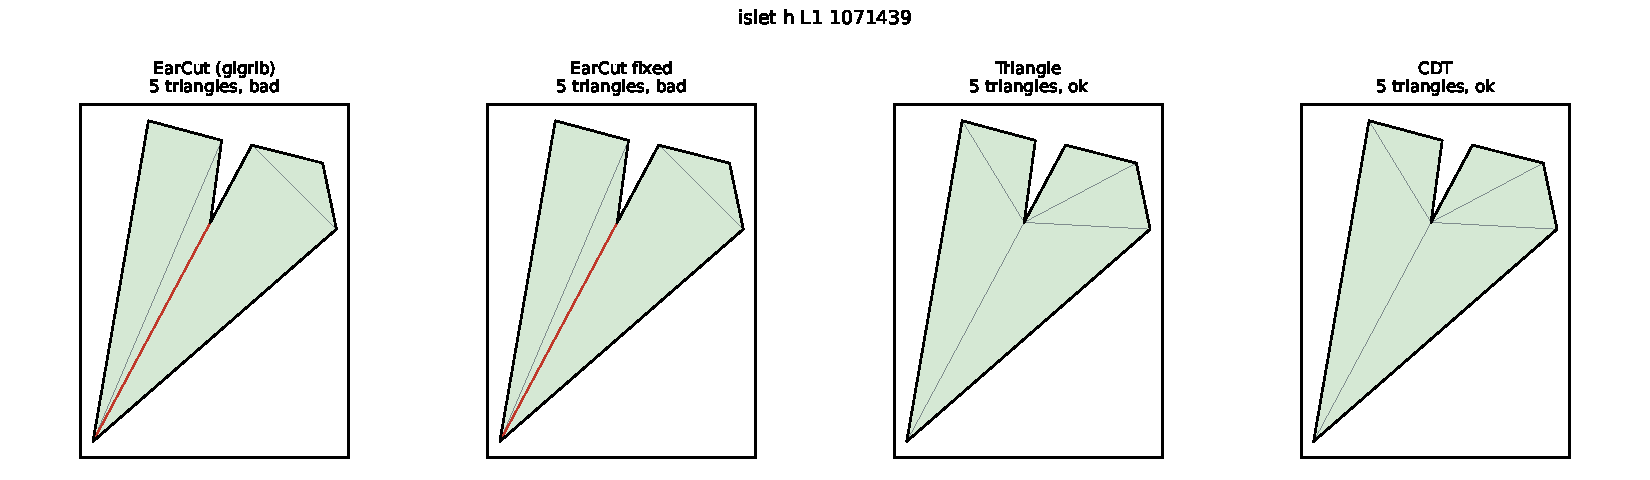
\includegraphics[width=\textwidth]{fig/cmp_case_islet_h_L1_1071439.pdf}
\caption{An islet of 2\,km near 64.7\,$^\circ$N 11.2\,$^\circ$E (GSHHS h L1, ring 1071439, 7
vertices). EarCut cuts the triangle (2,\,6,\,5), whose vertices are collinear to less than a metre;
its area is $-1.4\times10^{-12}$\,sr (57\,m$^2$), inverted. Triangle and CDT, which use exact
predicates in double precision, are correct.}
\label{fig:islet}
\end{figure}

Figure~\ref{fig:islet} shows a typical case. EarCut computes its geometric tests in single
precision: one float ulp of longitude or latitude is about 0.8\,m at 1.1\,rad. When three
consecutive vertices are collinear to within that, the test of convexity can take the wrong sign,
and an inverted ear is cut. Of the 78 polygons with inverted triangles (EarCut as in glgrib, all files), 73 have less than
2\,000\,m$^2$ inverted (median 94\,m$^2$), invisible on a globe; the largest reach
$2.5\times10^{4}$\,m$^2$ (GSHHS h L1), $5.2\times10^{4}$\,m$^2$ (Natural Earth 10m lakes) and,
for EarCut fixed, $9.7\times10^{4}$\,m$^2$ (i L1). The probable cause, single precision, has not been verified by a double-precision
build of EarCut.

The other EarCut failures are incomplete triangulations: the OpenMP early stop on rivers (13 rings
in h L2, described in \code{earcut.pdf}) and Honshu (Figure~\ref{fig:honshu}).

\begin{figure}[!htb]
\centering
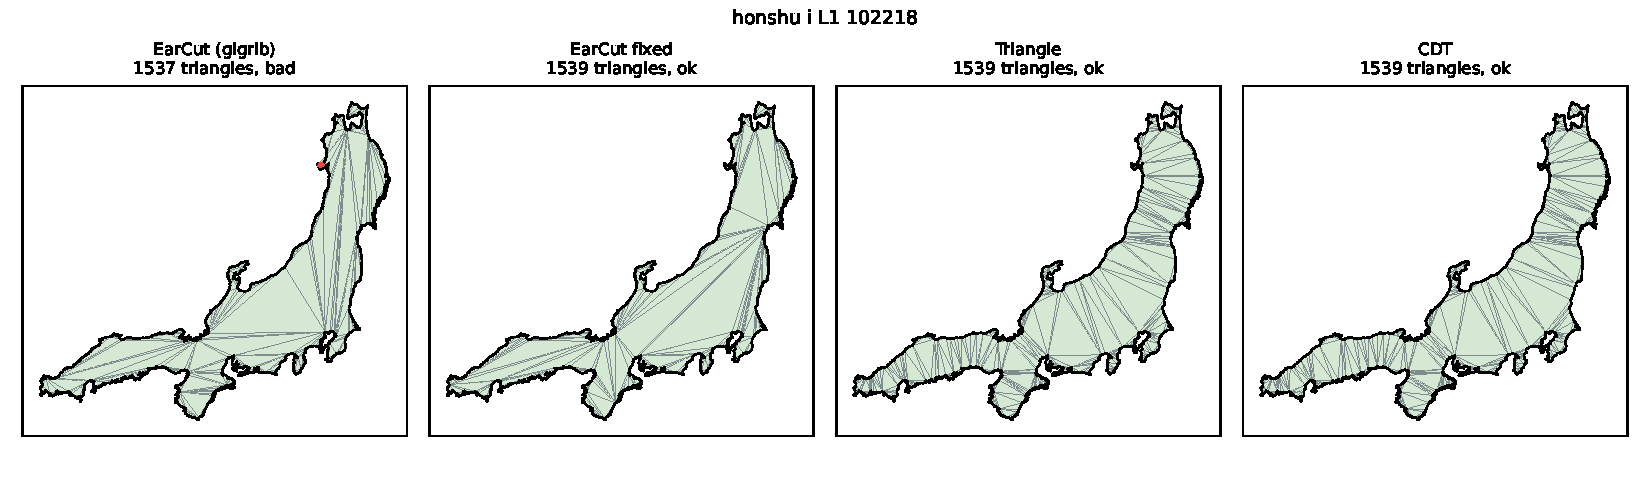
\includegraphics[width=\textwidth]{fig/cmp_case_honshu_i_L1_102218.pdf}
\caption{Honshu (GSHHS i L1, 1\,541 vertices). EarCut as in glgrib leaves two triangles out (red);
the other three methods are correct. The Delaunay triangulations avoid the long thin triangles
of ear cutting.}
\label{fig:honshu}
\end{figure}

\subsection{A new EarCut bug: \code{getLatRange}}\label{sec:latrange}

On Natural Earth 10m land, EarCut aborts in the spatial index (\code{xy2node\_t::iterator}, an
\code{abort ()} on an index out of range). The latitude range passed to the iterator was
$[-9.1\times10^{32}, 3.1\times10^{-41}]$. It comes from
\code{getLatRange (lonlat1, lonlat2, \&latmin, \&latmax)} (\code{EarCut.cc}, line 342):

\begin{lstlisting}[language=C++]
  float np = glm::length (p);   // p = p1 x p2
  if (np == 0.0f)
    {
      if (glm::dot (p1, p2) < 0.0f)
        zmax = 1.0f;
      return;                    // latmin and latmax are not set
    }
\end{lstlisting}

\noindent When the two points coincide (or are antipodal), the function returns without writing
its results, and the caller uses uninitialised values. Natural Earth closes Antarctica with a run
of points along latitude $-90^\circ$, which are the same point on the sphere; GSHHS has no such
run, which is why the bug did not show before. The fix is to set
\code{*latmin = asin (zmin); *latmax = asin (zmax);} before returning. EarCut fixed did not abort
on this file, but since the values are uninitialised this is no guarantee.

\subsection{Invalid rings}\label{sec:invalid}

\begin{figure}[!htb]
\centering
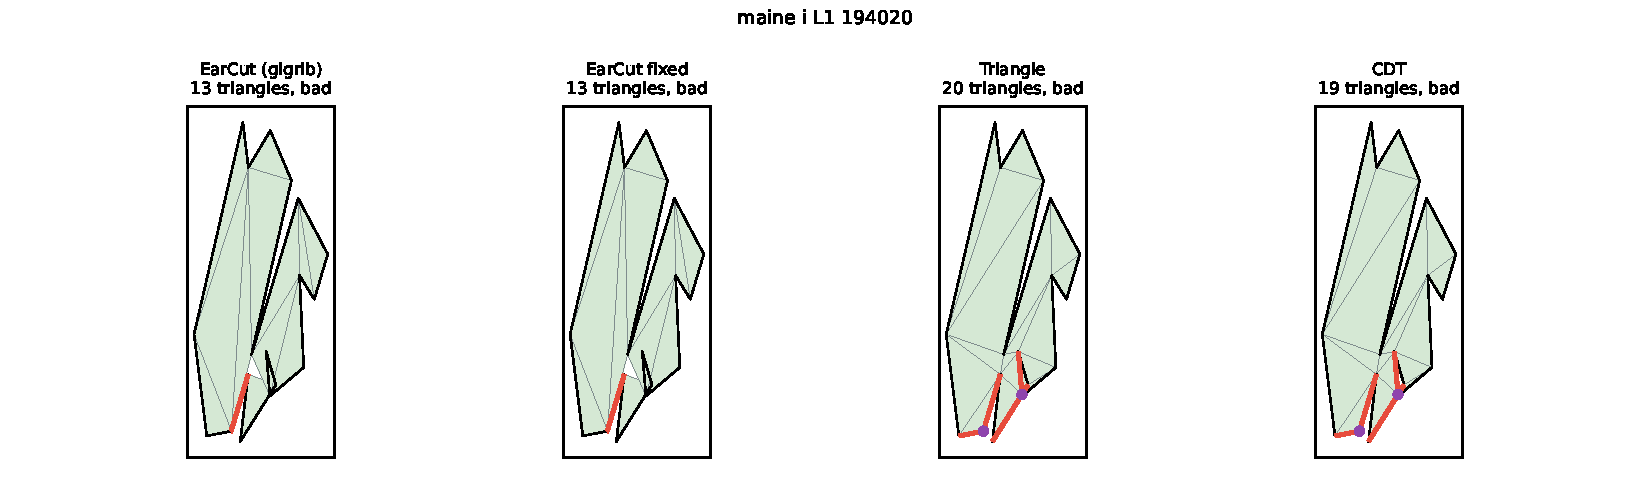
\includegraphics[width=\textwidth]{fig/cmp_case_maine_i_L1_194020.pdf}
\caption{The Maine island (GSHHS i L1, ring 194020) crosses itself twice. EarCut leaves a hole
(4 triangles missing). Triangle and CDT insert a vertex at each crossing (purple) and fill the
ring; the edges they split are drawn in red.}
\label{fig:maine}
\end{figure}

On self-crossing rings (Figure~\ref{fig:maine}), the area of a ``correct'' triangulation is not
defined. Triangle and CDT insert a vertex at each crossing and fill the ring by the even--odd rule
(CDT) or from the outside in (Triangle); their area differs from the ring's signed area by the
area of the small loops, which is why these rings count as failures in Table~\ref{tab:robust}.
EarCut leaves part of the ring empty. The same happens on the near-duplicate ring (i L2 81960: two
of its four points $10^{-6}$\,rad apart, the edges cross).

In the Americas polygon of Natural Earth 3.0.1 (ring 210702, 129\,579 vertices, 582 lakes as
holes), two lakes share an edge and ten points are shared between lakes. The shared edge belongs
to two holes and cancels out; the area is exact, but two edges are reported missing.

A ring that touches itself at a vertex (Natural Earth 10m lakes, ring 38847, with one point
repeated, not consecutively) is handled by CDT but not by Triangle, which leaves two extra
triangles in the pinched region; EarCut's result there is complete but its smallest angle is
below $5^\circ$ for half of the triangles (\S\ref{sec:quality}).

\subsection{Antarctica}\label{sec:antarctica}

GSHHS splits Antarctica into two halves, each closed along the meridian $0^\circ$/$180^\circ$
through the South Pole with two pole points, $(180^\circ, -90^\circ)$ and
$(0^\circ, -90^\circ)$. After the conversion to float, $\cos(-\pi/2)$ is not zero, so these two
points are about $10^{-7}$\,rad apart instead of being equal; the tiny edge between them crosses
its neighbours. Triangle and CDT add one vertex there, with an area error of $10^{-9}$. EarCut is
correct on the crude rings, but misses 18 triangles on GSHHS h L6 ring 17477.

Natural Earth closes Antarctica differently: a \emph{slit} along the antimeridian, from the coast
at $-84.35^\circ$ to the pole, traversed once on each side ($+180^\circ$ and $-180^\circ$), and at
10m a run of 724 points along $-90^\circ$. Triangle and CDT add a vertex where the slit meets the
coast and a few at the pole (Figure~\ref{fig:neant}).

\begin{figure}[!htb]
\centering
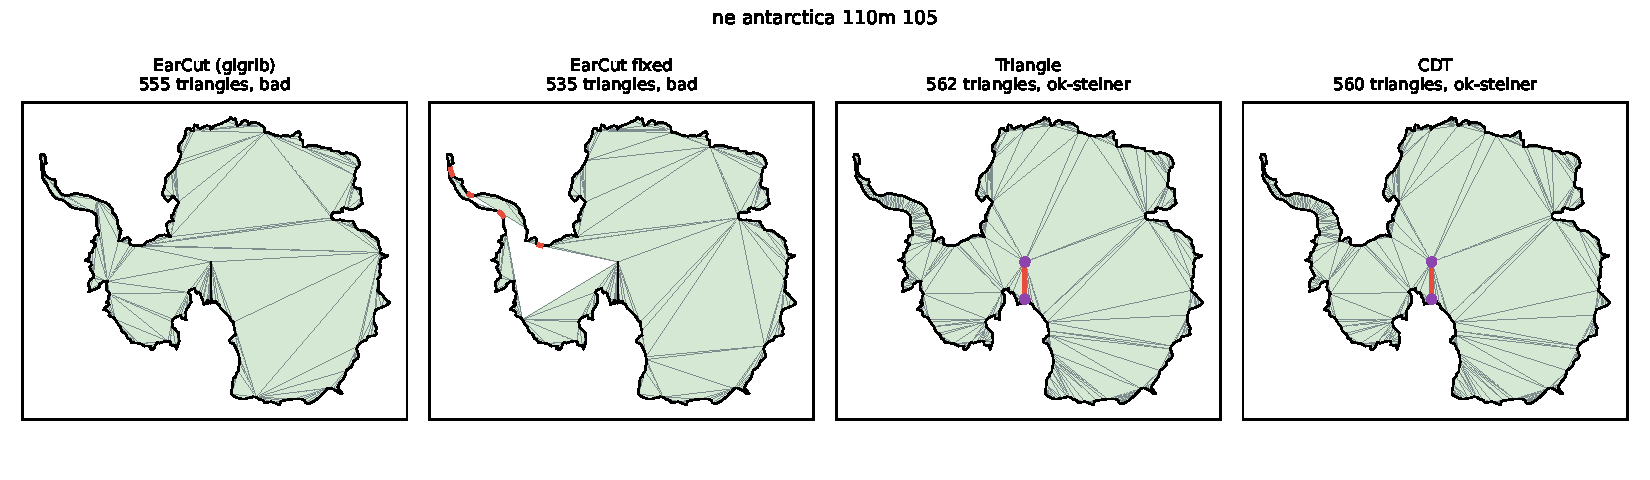
\includegraphics[width=\textwidth]{fig/cmp_case_ne_antarctica_110m_105.pdf}
\caption{Antarctica in Natural Earth 5.1.1, 1:110 million (ring 105, 558 vertices), seen from
above the pole.}
\label{fig:neant}
\end{figure}

\subsection{An exact detector of invalid rings}\label{sec:detector}

CDT no-X refuses a polygon as soon as two of its edges cross or overlap, using exact predicates.
Over all files it refused exactly: every Antarctica ring through the pole (GSHHS L5 and L6, at
all resolutions, and the Natural Earth Antarctica), the Maine island at i and h, the
near-duplicate ring, and nothing else. Its cost is that of a triangulation. This is the check
needed by the offline cleaning tool considered in \code{gshhs-data-notes.md}.

\subsection{Natural Earth compared with GSHHS}

Apart from the way Antarctica is closed, neither data set has self-crossing rings at the coarser
resolutions; GSHHS has two (Maine, near-duplicate) at i and h, Natural Earth 5.1.1 none.
Natural Earth has other defects:

\begin{itemize}
\item its lake files repeat points: 1\,164 consecutive duplicates in 443 of the 465 rings of 50m
  lakes (harmless once merged), and one ring touching itself (10m);
\item the version shipped with Magics (3.0.1) contains 248 rings of zero area at 10m.
\end{itemize}

\noindent Both data sets therefore need the same handling: merge identical points, ignore
zero-area rings, and treat Antarctica's closure specially or use a method that handles it.

\section{Performance}

\subsection{Whole layers}

Table~\ref{tab:time} and Figure~\ref{fig:layers} give the wall time to triangulate whole layers,
best of three runs, on an Intel Core Ultra 7 155U (14 threads), gcc 13.3, \code{-O2}.
``1 thread'' uses \code{OMP\_NUM\_THREADS=1}; ``parallel'' processes the polygons like
\code{Land::layer\_t::triangulate}: rings of 300 points or more one after the other (EarCut then
uses OpenMP inside them), smaller ones in a parallel loop. Times include the projection for
Triangle and CDT, and exclude reading the file and the checks.

\begin{table}[!htb]
\centering\small
\begin{tabular}{lrrrrrrrr}
\toprule
 & \multicolumn{4}{c}{1 thread} & \multicolumn{4}{c}{parallel (14 threads)} \\
\cmidrule(lr){2-5}\cmidrule(lr){6-9}
file & EarCut & fixed & Triangle & CDT & EarCut & fixed & Triangle & CDT \\
\midrule
GSHHS c L1 & 0.011 & 0.008 & \textbf{0.006} & 0.009 & 0.008 & \textbf{0.005} & 0.005 & 0.006 \\
GSHHS i L1 & 0.396 & 0.558 & \textbf{0.226} & 0.370 & 0.207 & 0.382 & \textbf{0.143} & 0.204 \\
GSHHS h L1 & 2.728 & 5.734 & \textbf{1.112} & 1.837 & 1.116 & 4.858 & \textbf{0.715} & 1.019 \\
GSHHS h L2 & 0.422 & 0.580 & \textbf{0.172} & 0.290 & 0.422 & 0.395 & \textbf{0.070} & 0.107 \\
NE 110m land & 0.006 & 0.005 & \textbf{0.005} & 0.008 & 0.010 & \textbf{0.005} & 0.005 & 0.007 \\
NE 50m land & 0.067 & 0.080 & \textbf{0.055} & 0.075 & 0.063 & 0.056 & \textbf{0.043} & 0.051 \\
NE 10m land & crash & 1.623 & 0.620 & \textbf{0.581} & crash & 1.476 & 0.524 & \textbf{0.417} \\
\bottomrule
\end{tabular}

\caption{Wall time (s) for whole layers. Bold: fastest method in each half of a row.}
\label{tab:time}
\end{table}

\begin{figure}[!htb]
\centering
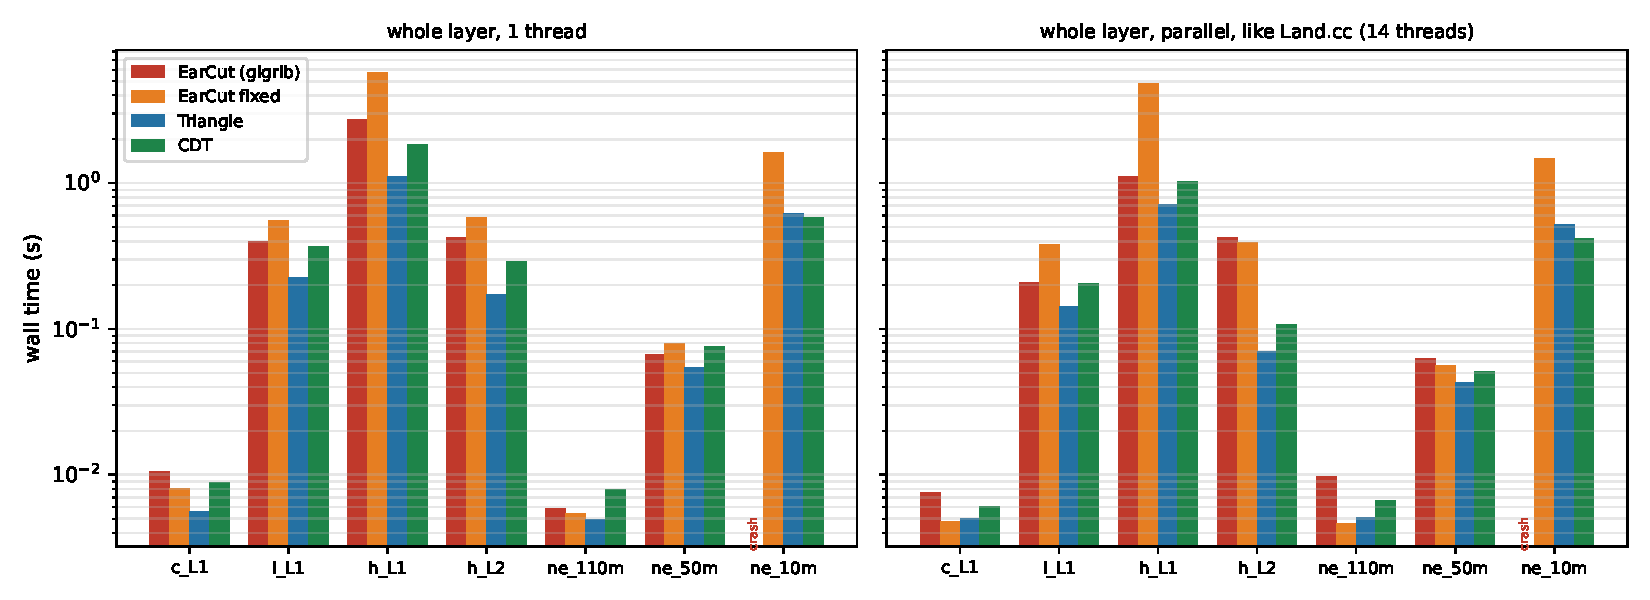
\includegraphics[width=\textwidth]{fig/cmp_layer_times.pdf}
\caption{Wall time for whole layers (log scale).}
\label{fig:layers}
\end{figure}

\begin{itemize}
\item \textbf{Triangle is the fastest} on GSHHS, 1.5 to 2.5 times faster than EarCut with one
  thread.
\item \textbf{CDT is as fast as EarCut or faster}: GSHHS h L1 takes 1.84\,s against 2.73\,s with
  one thread, 1.02\,s against 1.12\,s in parallel; h L2 (rivers and lakes), 0.11\,s against
  0.42\,s in parallel.
\item \textbf{EarCut fixed is twice as slow as EarCut} on h L1 (5.7\,s). Separate runs of the
  instrumented EarCut show that the transposed rotation alone causes the slowdown (Eurasia: 0.34\,s
  $\to$ 1.35\,s); the serial passes cost nothing with one thread. The reason has not been
  investigated; the reflex-vertex index probably behaves differently once rings sit on the equator.
\item Triangle keeps global state (a random seed, among others) and is not thread-safe. Its
  parallel runs gave identical, correct results three times out of three, which proves nothing;
  CDT objects are independent and safe to use in parallel.
\end{itemize}

\noindent Peak memory of the whole process for GSHHS h L1 (1.5 million vertices), measured with
\code{/usr/bin/time -v}: EarCut 60\,MB, CDT 81\,MB, Triangle 99\,MB.

\subsection{Time per ring}

\begin{figure}[!htb]
\centering
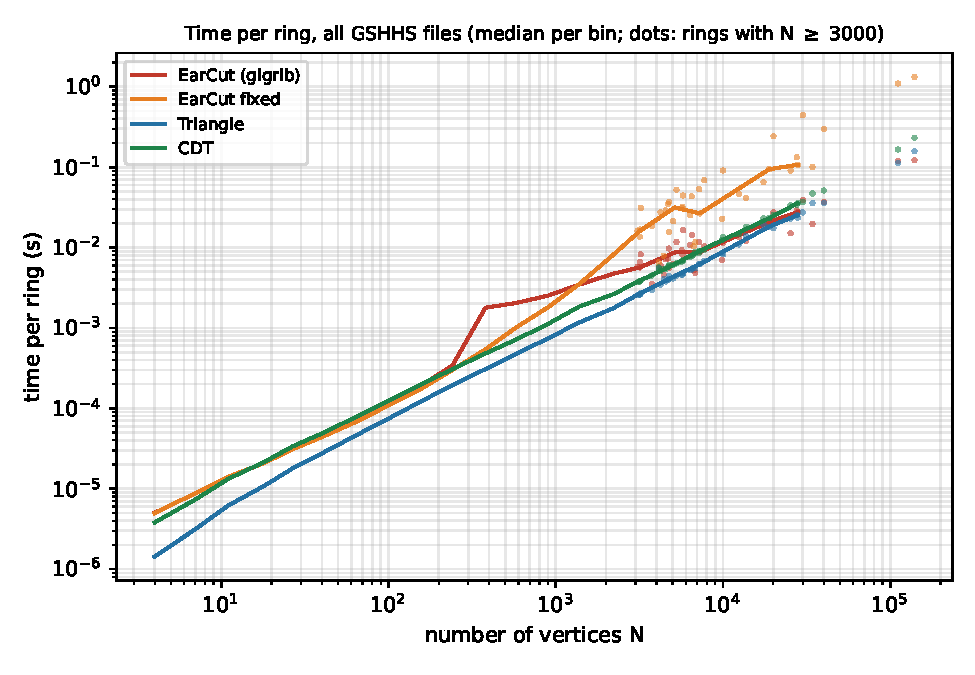
\includegraphics[width=0.8\textwidth]{fig/cmp_time_vs_n.pdf}
\caption{Time per ring against its number of vertices, all GSHHS files (from the runs with
checks, polygons one after the other, so EarCut uses OpenMP inside rings of 300 points or more).}
\label{fig:timen}
\end{figure}

Figure~\ref{fig:timen} shows that all methods grow roughly like $N$ to $N\log N$ for land rings.
EarCut's time jumps by a factor of 5 at $N=300$, where glgrib switches OpenMP on inside the ring:
for rings of 300 to a few thousand points, the cost of starting 14 threads exceeds the work.
The scatter of EarCut fixed at large $N$ reflects the slowdown described above.

\section{Triangle quality}\label{sec:quality}

glgrib fills polygons with a uniform colour, so thin triangles are not visible. They would matter
for other uses (interpolation, texturing, line rendering along the coast). Table~\ref{tab:quality}
gives the smallest angle of each triangle for some of the polygons drawn in this report.

\begin{table}[!htb]
\centering\small
\begin{tabular}{lrrrrrr}
\toprule
 & \multicolumn{3}{c}{EarCut} & \multicolumn{3}{c}{CDT} \\
\cmidrule(lr){2-4}\cmidrule(lr){5-7}
polygon & median & $<5^\circ$ & $<1^\circ$ & median & $<5^\circ$ & $<1^\circ$ \\
\midrule
Honshu (GSHHS i L1)                & 14.8$^\circ$ & 23.0\,\% & 7.2\,\% & 21.4$^\circ$ & 8.3\,\% & 0.1\,\% \\
Ob--Irtysh (GSHHS i L2)            & 12.3$^\circ$ & 13.0\,\% & 2.9\,\% & 23.8$^\circ$ & 0.4\,\% & 0.0\,\% \\
Maine island (GSHHS h L1)          & 14.0$^\circ$ & 13.8\,\% & 3.7\,\% & 27.2$^\circ$ & 2.7\,\% & 0.0\,\% \\
Antarctica (NE 110m)               & 7.8$^\circ$  & 35.7\,\% & 11.5\,\% & 12.1$^\circ$ & 17.0\,\% & 0.9\,\% \\
pinched lake (NE 10m lakes)        & 4.7$^\circ$  & 51.7\,\% & 22.4\,\% & 19.0$^\circ$ & 10.3\,\% & 1.7\,\% \\
\bottomrule
\end{tabular}
\caption{Smallest angle per triangle: median, and share of triangles below $5^\circ$ and $1^\circ$.
Triangle gives the same values as CDT to within 1\,\%. All values: \code{tables/quality.txt}.}
\label{tab:quality}
\end{table}

\begin{figure}[!htb]
\centering
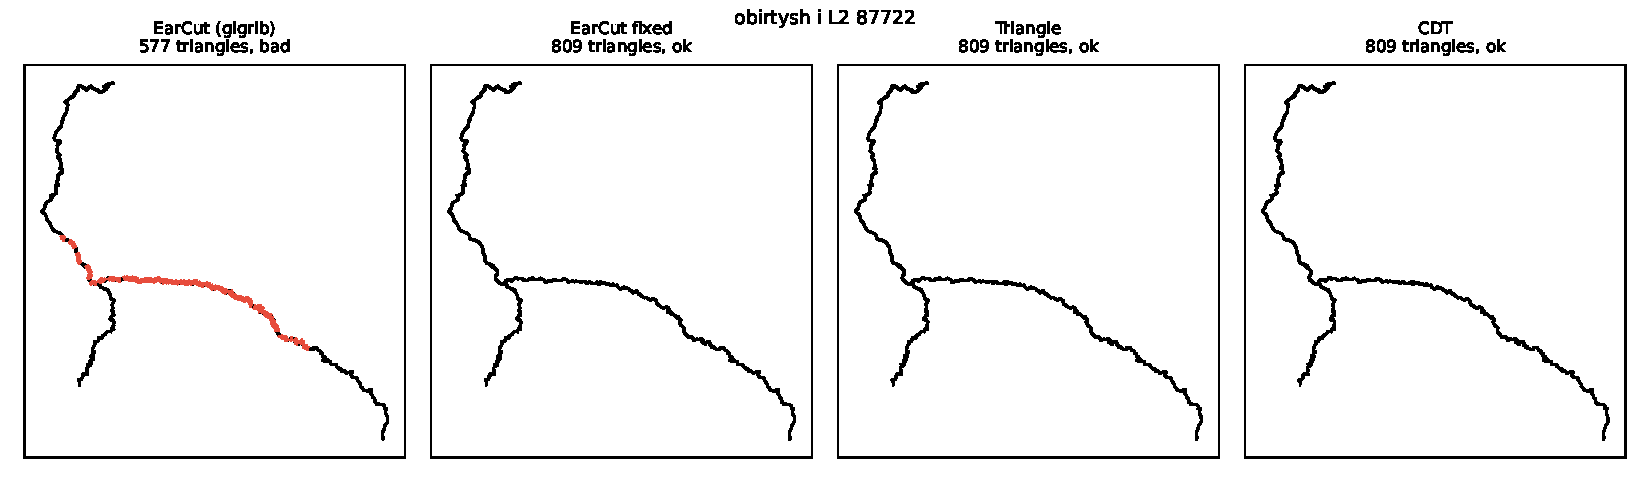
\includegraphics[width=\textwidth]{fig/cmp_case_obirtysh_i_L2_87722.pdf}
\caption{The Ob--Irtysh river (GSHHS i L2, 811 vertices). EarCut as in glgrib stops early (OpenMP,
577 of 809 triangles); EarCut fixed completes it; Triangle and CDT triangulate it with far fewer
thin triangles.}
\label{fig:river}
\end{figure}

\section{What adopting CDT in glgrib would involve}

\begin{itemize}
\item \textbf{Projection}: per polygon, a stereographic projection from the antipode of the mean of
  the ring, and the reverse projection of any added vertex (the driver does this in 40 lines).
  Long edges (Antarctica's meridians) should be subdivided first.
\item \textbf{Identical points}: CDT refuses duplicate vertices; they must be merged
  (\code{CDT::RemoveDuplicatesAndRemapEdges}) and the triangles mapped back.
\item \textbf{Steiner points}: only invalid rings get them (43 in total with CDT over all files:
  Antarctica, the Maine island, the near-duplicate ring). Either \code{Land::layer\_t} appends them to the
  vertex buffer, or such rings are rejected (CDT no-X) and repaired in the data.
\item \textbf{Holes}: CDT handles them, so Natural Earth land and lakes could be used as they are.
\item \textbf{Dependency}: CDT is a header-only C++ library under MPL-2.0, compatible with GPLv3.
\end{itemize}

\section{Recommendation}

\begin{enumerate}
\item \textbf{Replace EarCut by CDT} (\code{TryResolve}, \code{eraseOuterTrianglesAndHoles}),
  using the stereographic projection described here and appending Steiner points to the vertex
  buffer. It is correct on all valid rings, never produces inverted triangles, handles holes,
  repeated points and the Antarctic closures, is at least as fast as EarCut, and gives better
  triangles.
\item \textbf{Use CDT no-X in the offline cleaning tool} to list the invalid rings of the data
  (\code{gshhs-data-notes.md}); there are only a handful in GSHHS outside Antarctica.
\item \textbf{If EarCut is kept}, fix \code{getLatRange} (\S\ref{sec:latrange}), the rotation and
  the OpenMP early stop (\code{earcut.pdf}), and switch OpenMP on only for much larger rings.
  Even then it leaves inverted slivers on about 1 ring in 2\,600 at i and h, and it is twice as
  slow with the rotation corrected.
\item \textbf{Natural Earth} is not clearly cleaner than GSHHS. Switching would only be worth it
  for other reasons (maintenance, licence, matching Magics' maps), and would need hole support,
  which CDT provides.
\end{enumerate}

\noindent Not done (optional items of the plan): synthetic test polygons (\S6.3 of the plan) and a
trial of CDT inside glgrib with rendered images (\S9).

\appendix
\section{How to reproduce}

From \code{share/doc/earcut}, download the libraries and data (not committed) into
\code{tools/ext}:

\begin{lstlisting}[language=bash]
mkdir -p tools/ext/triangle tools/ext/cdt tools/ext/naturalearth
cd tools/ext/triangle
curl -sSfLO https://www.netlib.org/voronoi/triangle.zip && unzip triangle.zip
cd ../../..
git clone --depth 1 --branch 2.1.0 \
    https://github.com/artem-ogre/CDT.git tools/ext/cdt/src
cd tools/ext/naturalearth
for s in 110m 50m 10m; do for f in land lakes; do
  curl -sSfLO https://naciscdn.org/naturalearth/$s/physical/ne_${s}_$f.zip
  unzip -o ne_${s}_$f.zip -d $s
done; done
cd ../../..
\end{lstlisting}

\noindent Versions used: \code{triangle.zip} SHA-256 \code{1766327add038495\ldots}; CDT 2.1.0
(commit \code{d66c2024}); Natural Earth 5.1.1; Magics commit \code{cb97794} for Natural Earth
3.0.1. Then:

\begin{lstlisting}[language=bash]
export MAGICS_NE=/path/to/magics/share/magics
./tools/make-comparison.sh /path/to/work
./tools/make-comparison-dumps.sh /path/to/work
# single-thread timings, 3 runs per file and method, into timings1/:
#   OMP_NUM_THREADS=1 tri_driver FILE METHOD nocheck all
python3 tools/summarize_comparison.py /path/to/work
python3 tools/tables_comparison.py /path/to/work tables
python3 tools/figs_comparison.py   /path/to/work fig
python3 tools/quality_comparison.py /path/to/work > tables/quality.txt
\end{lstlisting}

\noindent The driver \code{tools/tri\_driver.cc} is built by \code{tools/build-tri-driver.sh}; it
links the unmodified \code{src/glGrib/EarCut.cc}, a \code{sed}'ed copy for EarCut fixed (in the
namespace \code{glGribFix}), Triangle (with \code{triexit} redirected to a \code{longjmp}, since
Triangle calls \code{exit} on errors) and CDT. No file of glgrib is modified. Usage:

\begin{lstlisting}
tri_driver file.shp METHOD [par] [nocheck] [noholes] [dump=dir]
           [rank ...|all|min=N]
METHOD = earcut | earcut-fix | triangle | triangle-Y | cdt | cdt-noX | cdt-outer
\end{lstlisting}

\noindent Two problems of the libraries found while writing the driver: Triangle with \code{-Y}
crashes (segmentation fault in \code{scoutsegment}) on rings with identical points, depending on
its random seed, so the driver merges identical points before calling it, as for CDT; and
Triangle's hole removal in the driver uses a point-in-polygon test per triangle, which is slow on
the Americas of Natural Earth 3.0.1 with 582 holes (14\,s) --- a cost of the driver, not of Triangle, which accepts a list of
hole points instead.

\end{document}
